\subsection*{НГУ-2.29}

\setcounter{equation}{0}

\begin{abstract}
В металлическом изолированном шаре радиуса $a$ имеется сферическая полость, в центре которой за-
креплен заряд $q_0$. Вне шара на расстоянии $\ell$ от его центра расположен второй заряд $q$. Найти силу действующую на заряд $q$.
\end{abstract}

\noindent \hrulefill
\\
\begin{wrapfigure}[6]{r}{0.30\textwidth}
	\raisebox{0pt}[\dimexpr\height-2\baselineskip\relax]{
	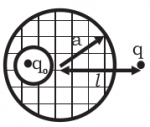
\includegraphics[width=0.30\textwidth]{pics/2.29-1.png}}
\end{wrapfigure}

\begin{wrapfigure}[6]{r}{0.30\textwidth}
	\raisebox{0pt}[\dimexpr\height-1\baselineskip\relax]{
	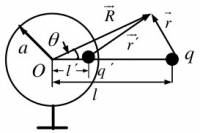
\includegraphics[width=0.30\textwidth]{pics/2.29-2.jpg}}
\end{wrapfigure}

В полости шара есть заряд $q_0$, который делает внутреннюю сторону шара заряд $-q_0$, в результате чего распределение заряда на внешней стороне ($q_0$) шара изменяется. Мы используем метод изображений, чтобы найти виртуальный заряд $q'$ вместо неравномерно распределенного заряда на внешней стороне шара .


Предположим, что существует виртуальный заряд $q'$. Заряд всего шара равен $q_0$, поэтому мы разделяем его на систему, состоящую из: 

* $q'$ расположен в длине $b$ от центра шара

* $q_0 - q'$ расположен в центре шара (чтобы не влиять на напряжение на поверхность шара). 

В данный момент сила приложена к $q$:

$$F = k \times q \times[\frac{q_0-q'}{\ell^2} + \frac{q'}{(\ell-\ell')^2}] 
 \qquad(1)$$

Согласно методу изображений, напряжение равно 0 в каждой точке на поверхности шара.

Потенциал в любой точке на поверхности шара равно:

$$\phi = \frac{k \times q'}{\sqrt{\ell'^2+a^2-2\ell'a \cos{\theta}}} + \frac{k \times q}{\sqrt{\ell^2+a^2-2\ell a \cos{\theta}}} = 0$$

$$\Longrightarrow q' = -q \times \frac{\sqrt{\ell'^2+a^2-2\ell' a \cos{\theta} }}{\sqrt{\ell^2+a^2-2\ell a \cos{\theta} }}$$

Так что приведенное выше выражение всегда истинно для каждого $\theta$:

$$\frac{\sqrt{\ell'^2+a^2-2\ell' a \cos{\theta} }}{\sqrt{\ell^2+a^2-2\ell a \cos{\theta} }} = const$$

$$\Longrightarrow \frac{\ell'^2 + a^2}{l^2 + a^2} = \frac{-2 \ell' a \cos{\theta}}{-2 \ell a \cos{\theta}} = \frac{\ell'}{\ell} = const$$

$$\Longrightarrow \ell' = \frac{a^2}{\ell} \qquad (2)$$

С другой стороны ($\theta = 0$):

$$\phi = \frac{kq'}{a-\ell'} + \frac{kq}{\ell -a}=0 \xrightarrow{} q' = -q \times \frac{a-\ell'}{\ell-a} = -q \times \frac{a}{\ell} \qquad (3)$$

Заменим $(2)$ и $(3)$ на $(1)$:

$$\Longrightarrow F = k \times [\frac{qq_0}{\ell^2} + \frac{q^2a}{\ell^3} - \frac{q^2a \ell}{(\ell^2-a^2)^2}]$$

\textbf{Ответ:}

$$F = k \times [\frac{qq_0}{\ell^2} + \frac{q^2a}{\ell^3} - \frac{q^2a \ell}{(\ell^2-a^2)^2}].$$





